\documentclass[border=5pt]{article}
\usepackage[utf8]{inputenc}
\usepackage{amsmath,amssymb,amsthm}
\usepackage{graphicx}
\usepackage{geometry}
\geometry{margin=1in}
\usepackage{hyperref}
\usepackage{tikz}
\usetikzlibrary{arrows.meta,positioning,calc,fit,decorations.pathmorphing}
\usetikzlibrary{knots,calc, hobby}

\begin{document}

\\
\\



    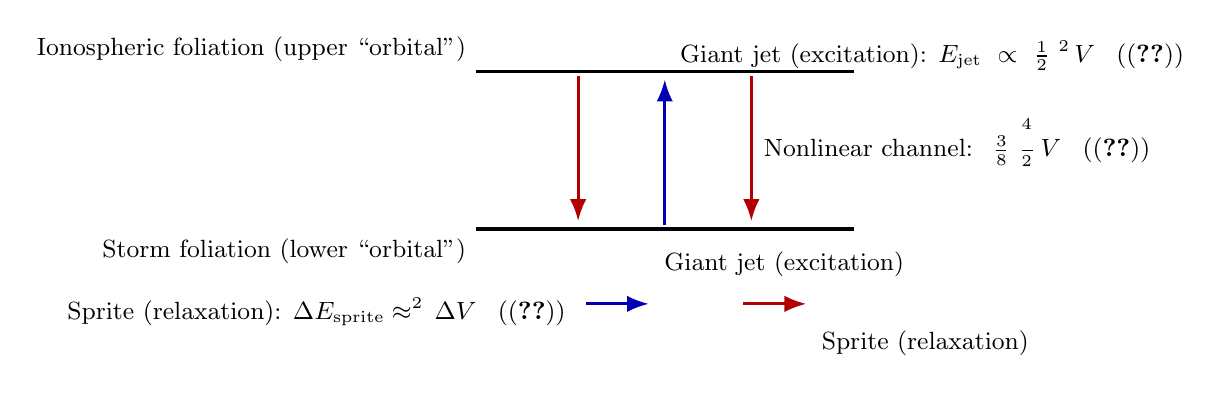
\begin{tikzpicture}[x=1cm,y=1cm,
        level/.style={line width=1.2pt},
        arrow/.style={-Latex, line width=1.1pt},
        jet/.style={arrow, blue!70!black},
        sprite/.style={arrow, red!70!black},
        label/.style={font=\small}
    ]

% Levels
    \draw[level] (-2.4,2.0) -- (2.4,2.0);
    \draw[level] (-2.4,0.0) -- (2.4,0.0);

% Level labels
    \node[label, above left] at (-2.4,2.0) {Ionospheric foliation (upper “orbital”)};
    \node[label, below left] at (-2.4,0.0) {Storm foliation (lower “orbital”)};

% Upward giant-jet excitation
    \draw[jet] (0.0,0.05) -- (0.0,1.90);
    \node[label, right=2pt] at (0.0,2.20) {Giant jet (excitation): $E_{\text{jet}}\ \propto\ \tfrac{1}{2}\,\rhof\,\vnorm^2\,V$ \, (\eqref{eq:jet})};

% Downward sprite relaxations (two channels)
    \draw[sprite] (-1.1,1.95) -- (-1.1,0.10);
    \node[label, left=1pt] at (-1.1,-1.05) {Sprite (relaxation): $\Delta E_{\text{sprite}}\approx \rhof \Ce^2\,\Delta V$ \, (\eqref{eq:sprite})};

    \draw[sprite] (1.1,1.95) .. controls (1.1,1.2) and (1.1,0.8) .. (1.1,0.10);
    \node[label, right=1pt, align=left] at (1.1,1.05) {Nonlinear channel: $\ \tfrac{3}{8}\,\rhof\,\dfrac{\vnorm^4}{\Ce^2}\,V$ \, (\eqref{eq:VAMseries})};

% Legend
    \begin{scope}[shift={(0,-0.95)}]
    \draw[jet] (-1.0,0) -- (-0.2,0); \node[label, right=2pt] at (-0.2,.5) {Giant jet (excitation)};
    \draw[sprite] (1.0,0) -- (1.8,0); \node[label, right=2pt] at (1.8,-.5) {Sprite (relaxation)};
    \end{scope}

    \end{tikzpicture}


    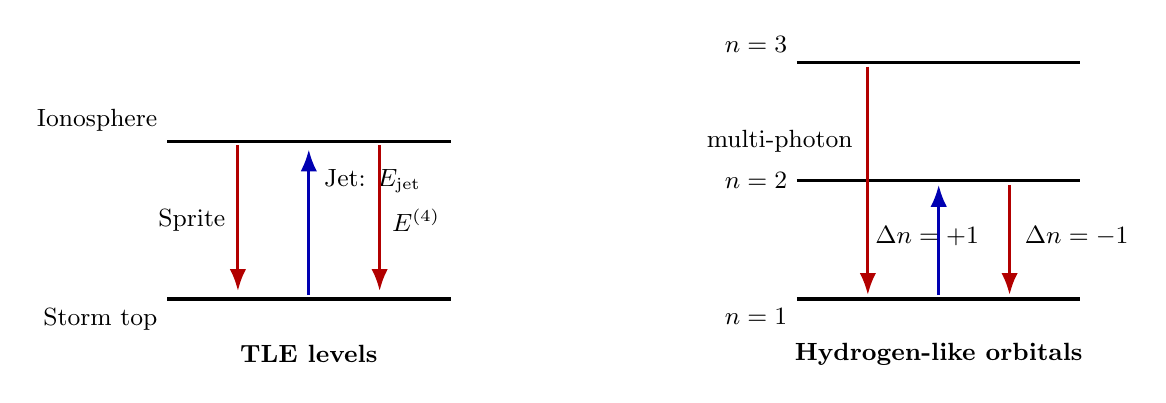
\begin{tikzpicture}[x=1cm,y=1cm,
        level/.style={line width=1.2pt},
        arrow/.style={-Latex, line width=1.1pt},
        jet/.style={arrow, blue!70!black},
        sprite/.style={arrow, red!70!black},
        label/.style={font=\small}
    ]

% --- Left: TLE levels ---
    \begin{scope}[shift={(-4,0)}]

% Levels
    \draw[level] (-1.8,2.0) -- (1.8,2.0);
    \draw[level] (-1.8,0.0) -- (1.8,0.0);

% Labels
    \node[label, above left] at (-1.8,2.0) {Ionosphere};
    \node[label, below left] at (-1.8,0.0) {Storm top};

% Jet upward
    \draw[jet] (0,0.05) -- (0,1.90);
    \node[label, right=2pt] at (0,1.5) {Jet: $E_{\text{jet}}$};

% Sprite down
    \draw[sprite] (-0.9,1.95) -- (-0.9,0.10);
    \node[label, left=1pt] at (-0.9,1.0) {Sprite};

% Quartic channel
    \draw[sprite] (0.9,1.95) .. controls (0.9,1.2) and (0.9,0.8) .. (0.9,0.10);
    \node[label, right=1pt] at (0.9,1.0) {$E^{(4)}$};

% Title
    \node[font=\small\bfseries] at (0,-0.7) {TLE levels};

    \end{scope}

% --- Right: Hydrogen-like orbitals ---
    \begin{scope}[shift={(4,0)}]

% Levels
    \draw[level] (-1.8,3.0) -- (1.8,3.0);
    \draw[level] (-1.8,1.5) -- (1.8,1.5);
    \draw[level] (-1.8,0.0) -- (1.8,0.0);

% Labels
    \node[label, above left] at (-1.8,3.0) {$n=3$};
    \node[label, left] at (-1.8,1.5) {$n=2$};
    \node[label, below left] at (-1.8,0.0) {$n=1$};

% Excitation arrow
    \draw[jet] (0,0.05) -- (0,1.45);
    \node[label, right=2pt] at (-1,0.8) {$\Delta n=+1$};

% Relaxation arrow
    \draw[sprite] (0.9,1.45) -- (0.9,0.05);
    \node[label, right=2pt] at (0.9,0.8) {$\Delta n=-1$};

% Multi-step downward
    \draw[sprite] (-0.9,2.95) .. controls (-0.9,2.2) and (-0.9,0.8) .. (-0.9,0.05);
    \node[label, left=2pt] at (-0.9,2) {multi-photon};

% Title
    \node[font=\small\bfseries] at (0,-0.7) {Hydrogen-like orbitals};

    \end{scope}

    \end{tikzpicture}



\end{document}
